% !TEX program = xelatex
\ifdefined\MASTERBOOK\else
\documentclass[UTF8,zihao=-4,oneside,openany]{ctexbook}

\usepackage[a4paper,top=20mm,bottom=22mm,left=19mm,right=19mm,headheight=24pt]{geometry}
\usepackage[table]{xcolor}
\usepackage{amsmath,amssymb,mathtools,bm}
\usepackage{siunitx}
\usepackage{booktabs,tabularx,array}
\usepackage{enumitem}
\usepackage{tikz}
\usetikzlibrary{arrows.meta,calc,patterns,angles,quotes}
\usepackage[most]{tcolorbox}
\usepackage{fancyhdr}
\usepackage{hyperref}

% ---------- restrained textbook theme ----------
\definecolor{Ink}{HTML}{202326}
\definecolor{DeepBlue}{HTML}{294E69}
\definecolor{Blue}{HTML}{47687D}
\definecolor{Gold}{HTML}{6E777D}
\definecolor{Green}{HTML}{5B6D76}
\definecolor{PaleBlue}{HTML}{F3F5F6}
\definecolor{RuleGray}{HTML}{D3D7DA}
\definecolor{TextGray}{HTML}{61686D}
\definecolor{SoftGray}{HTML}{F6F6F6}

\color{Ink}
\sisetup{
  per-mode=symbol,
  inter-unit-product=\ensuremath{{}\cdot{}},
  exponent-product=\times
}

\hypersetup{
  colorlinks=true,
  linkcolor=DeepBlue,
  urlcolor=Blue,
  pdftitle={高中物理竞赛一轮讲义样章：函数、微积分与物理变化率},
  pdfsubject={高中物理竞赛一轮资料重排样章},
  pdfauthor={物理竞赛一轮资料编写组}
}

\setlength{\parindent}{2em}
\setlength{\parskip}{0.25em}
\setlist{nosep,leftmargin=2em}
\setcounter{secnumdepth}{3}
\setcounter{tocdepth}{2}
\numberwithin{equation}{section}
\counterwithin{table}{section}
\allowdisplaybreaks[2]
\emergencystretch=2em

\ctexset{
  chapter={
    format=\raggedright\LARGE\bfseries\color{Ink},
    titleformat=\LARGE\bfseries\color{Ink},
    beforeskip=0pt,
    afterskip=18pt
  },
  section={
    format=\Large\bfseries\color{DeepBlue},
    beforeskip=1.8ex,
    afterskip=1.0ex
  },
  subsection={
    format=\large\bfseries\color{Ink},
    beforeskip=1.5ex,
    afterskip=0.8ex
  },
  subsubsection={
    format=\normalsize\bfseries\color{Ink}
  }
}

\pagestyle{fancy}
\fancyhf{}
\fancyhead[L]{\small\color{TextGray}高中物理竞赛一轮讲义}
\fancyhead[R]{\small\color{TextGray}第一章\quad 数学与物理工具}
\fancyfoot[C]{\small\color{TextGray}\thepage}
\renewcommand{\headrulewidth}{0.4pt}
\renewcommand{\headrule}{\hbox to\headwidth{\color{RuleGray}\leaders\hrule height \headrulewidth\hfill}}

\newcommand{\dd}{\mathop{}\!\mathrm{d}}
\newcommand{\e}{\mathrm e}
\newcommand{\vect}[1]{\bm{#1}}
\newcommand{\uvec}[1]{\hat{\vect{#1}}}
\newcommand{\order}[1]{\mathcal O\!\left(#1\right)}

\newtcolorbox[auto counter,number within=section]{examplebox}[2][]{
  enhanced,breakable,
  colback=white,colframe=RuleGray,
  boxrule=0.5pt,arc=0mm,
  title={例题~\thetcbcounter\quad #2},fonttitle=\bfseries,
  coltitle=Ink,colbacktitle=PaleBlue,
  borderline west={1.4pt}{0pt}{DeepBlue},
  #1
}

\newtcolorbox{methodbox}[1]{
  enhanced,breakable,
  colback=PaleBlue,colframe=RuleGray,
  boxrule=0.5pt,arc=0mm,
  title={方法：#1},fonttitle=\bfseries,
  coltitle=Ink,colbacktitle=PaleBlue,
  borderline west={1.2pt}{0pt}{DeepBlue}
}

\newtcolorbox{warningbox}[1]{
  enhanced,breakable,
  colback=SoftGray,colframe=RuleGray,
  boxrule=0.5pt,arc=0mm,
  title={易错提醒：#1},fonttitle=\bfseries,
  coltitle=Ink,colbacktitle=SoftGray,
  borderline west={1.2pt}{0pt}{TextGray}
}

\tikzset{
  vector/.style={-{Latex[length=2.5mm]},very thick,draw=DeepBlue},
  axis/.style={-{Latex[length=2mm]},thin,draw=TextGray},
  curve/.style={very thick,draw=DeepBlue},
  guide/.style={densely dashed,draw=TextGray},
  tangent/.style={thick,draw=TextGray},
  secant/.style={thick,draw=DeepBlue}
}

\begin{document}

\pagenumbering{arabic}
\setcounter{page}{1}
\setcounter{chapter}{0}
\chapter{数学与物理工具}
\setcounter{section}{2}
\fi
\ifdefined\MASTERBOOK\clearpage\fi
\section{函数、微积分与物理变化率}

物理量之间的关系常常不是一个孤立的公式，而是一条完整的函数曲线。速度是位置随时间
的变化率，加速度是速度的变化率；反过来，已知每一时刻的速度，要得到一段时间内的位移，
就必须把许多个极短时间内的位移累加起来。导数和积分分别描述这两种互逆的过程。

本节不追求抽象的微积分体系，而从物理问题需要的三个动作出发：求变化率、研究局部行为、
把微小贡献累加成整体结果。推导中将明确写出自变量、积分限和物理单位，使数学运算始终
对应具体的物理意义；在掌握乘积法则和链式法则后，还将推导平面极坐标中的速度与加速度。

{\small\color{TextGray}\noindent\textbf{题源说明：}本节例题为本讲义依据微积分、约束运动、
连续分布和极坐标运动的经典模型自编，未逐字取自特定竞赛原题。\par}

\subsection{函数图像中的物理信息}

若物理量 $y$ 由物理量 $x$ 决定，可以写作 $y=f(x)$。定义域说明哪些 $x$ 在当前模型中
有意义，函数值说明对应状态下 $y$ 的大小。图像上的横、纵坐标必须连同单位一起理解：
同一组数据若改变坐标比例，曲线看起来会变陡或变缓，但它所表示的物理关系并未改变。

取曲线上两点 $P(x,f(x))$、$Q(x+\Delta x,f(x+\Delta x))$，割线斜率为
\begin{equation}
  \frac{\Delta y}{\Delta x}
  =\frac{f(x+\Delta x)-f(x)}{\Delta x}.
  \label{eq:average-rate}
\end{equation}
它表示从 $x$ 到 $x+\Delta x$ 这一区间内的平均变化率。斜率本身通常带有单位：
\[
  \left[\frac{\Delta y}{\Delta x}\right]=\frac{[y]}{[x]}.
\]
例如位置—时间图像斜率的单位是速度单位，压强—体积图像下方面积的单位则是能量单位。

\begin{center}
\begin{tikzpicture}[x=1.05cm,y=0.78cm]
  \draw[axis] (-0.2,0)--(6.4,0) node[right] {$x$};
  \draw[axis] (0,-0.2)--(0,5.2) node[above] {$y$};
  \draw[curve,domain=0.35:5.8,samples=80]
    plot (\x,{0.14*(\x-1.0)*(\x-1.0)+0.65});
  \coordinate (P) at (2.2,{0.14*(2.2-1.0)*(2.2-1.0)+0.65});
  \coordinate (Q) at (5.0,{0.14*(5.0-1.0)*(5.0-1.0)+0.65});
  \fill[Ink] (P) circle (1.5pt) node[above left] {$P$};
  \fill[Ink] (Q) circle (1.5pt) node[above right] {$Q$};
  \draw[secant] ($(P)!-0.35!(Q)$)--($(P)!1.25!(Q)$);
  \draw[tangent] ($(P)+(-1.2,-0.40)$)--($(P)+(1.4,0.47)$);
  \draw[guide] (P)--(P|-0,0) node[below,fill=white] {$x$};
  \draw[guide] (Q)--(Q|-0,0) node[below,fill=white] {$x+\Delta x$};
  \node[TextGray] at (4.95,1.8) {割线};
  \node[TextGray] at (1.25,1.7) {切线};
\end{tikzpicture}
\end{center}

当 $Q$ 沿曲线趋近 $P$ 时，割线趋近 $P$ 点的切线，平均变化率也趋近该点的瞬时变化率。
这正是导数的几何来源。

\subsection{从平均变化率到导数}

函数 $f(x)$ 在 $x$ 处的导数定义为
\begin{equation}
  f'(x)=\frac{\dd f}{\dd x}
  =\lim_{\Delta x\to0}
  \frac{f(x+\Delta x)-f(x)}{\Delta x}.
  \label{eq:derivative-definition}
\end{equation}
极限中的 $\Delta x$ 趋近于零但不先取零，因此分母始终不是零。导数描述的是一点附近的
局部规律，而不是用一个有限时间段的平均量代替瞬时量。

对直线运动，位置为 $x(t)$，于是
\begin{equation}
  v(t)=\frac{\dd x}{\dd t},
  \qquad
  a(t)=\frac{\dd v}{\dd t}=\frac{\dd^2x}{\dd t^2}.
  \label{eq:kinematic-derivatives}
\end{equation}
由导数单位立即得到
\[
  [v]=\frac{\mathsf L}{\mathsf T},
  \qquad
  [a]=\frac{\mathsf L}{\mathsf T^2}.
\]
同样，若 $F(x)$ 是弹性体的拉力—形变关系，则局部劲度
$k(x)=\dd F/\dd x$；若 $Q(T)$ 是吸热量—温度关系，则热容
$C(T)=\dd Q/\dd T$。导数所描述的“变化率”可以出现在各种物理量之间，并不限于时间。

\paragraph{幂函数求导}
从定义出发，对正整数 $n$，利用二项式展开
\begin{align*}
  \frac{(x+\Delta x)^n-x^n}{\Delta x}
  &=\frac{nx^{n-1}\Delta x+\binom n2x^{n-2}(\Delta x)^2+\cdots}{\Delta x}\\
  &=nx^{n-1}+\binom n2x^{n-2}\Delta x+\cdots.
\end{align*}
令 $\Delta x\to0$，所有含 $\Delta x$ 的项消失，得到
\begin{equation}
  \frac{\dd}{\dd x}x^n=nx^{n-1}.
  \label{eq:power-rule}
\end{equation}
这一结论可进一步推广到一般实数指数允许的范围。

\paragraph{乘积法则}
设 $f,g$ 都可导。把乘积的增量拆成两部分：
\begin{align*}
  &f(x+\Delta x)g(x+\Delta x)-f(x)g(x)\\
  &=[f(x+\Delta x)-f(x)]g(x+\Delta x)
   +f(x)[g(x+\Delta x)-g(x)].
\end{align*}
除以 $\Delta x$ 并取极限，利用可导函数连续，$g(x+\Delta x)\to g(x)$，于是
\begin{equation}
  \frac{\dd}{\dd x}(fg)=f'g+fg'.
  \label{eq:product-rule}
\end{equation}

\paragraph{链式法则}
若 $y=f(u)$、$u=g(x)$，令 $\Delta u=g(x+\Delta x)-g(x)$。在 $\Delta u\ne0$ 时
\[
  \frac{\Delta y}{\Delta x}
  =\frac{f(u+\Delta u)-f(u)}{\Delta u}
   \frac{\Delta u}{\Delta x}.
\]
取 $\Delta x\to0$，便有
\begin{equation}
  \frac{\dd y}{\dd x}
  =\frac{\dd y}{\dd u}\frac{\dd u}{\dd x}.
  \label{eq:chain-rule}
\end{equation}
链式法则的要点是沿依赖关系逐层求变化率，不能只对最外层函数求导。

常用初等函数的导数为
\begin{table}[htbp]
\centering
\caption{常用求导结果}
\rowcolors{2}{PaleBlue}{white}
\begin{tabularx}{0.88\textwidth}{>{\centering\arraybackslash}X >{\centering\arraybackslash}X >{\centering\arraybackslash}X}
\toprule
$f(x)$ & $f'(x)$ & 条件或说明 \\
\midrule
$C$ & $0$ & $C$ 为常量 \\
$x^n$ & $nx^{n-1}$ & 在函数有定义处 \\
$\sin x$ & $\cos x$ & $x$ 以弧度表示 \\
$\cos x$ & $-\sin x$ & $x$ 以弧度表示 \\
$\e^x$ & $\e^x$ & 指数自变量无量纲 \\
$\ln x$ & $1/x$ & $x>0$ \\
\bottomrule
\end{tabularx}
\end{table}

以 $\sin x$ 为例，和角公式给出
\[
  \frac{\sin(x+h)-\sin x}{h}
  =\sin x\frac{\cos h-1}{h}+\cos x\frac{\sin h}{h}.
\]
利用 $\lim_{h\to0}(\sin h/h)=1$、$\lim_{h\to0}[(\cos h-1)/h]=0$，便得到
$(\sin x)'=\cos x$。这里若角度不用弧度，极限中会额外出现单位换算系数。

\begin{examplebox}{衰减振动的速度与加速度}
质点的位置满足
\[
  x(t)=A\e^{-\beta t}\cos\omega t,
\]
其中 $A$ 为振幅常量，$\beta>0$，$\omega>0$。求速度和加速度。

\tcblower
$\e^{-\beta t}$ 与 $\cos\omega t$ 都随时间变化，必须使用乘积法则；对复合自变量
$-\beta t$、$\omega t$ 还要使用链式法则：
\begin{align*}
  v(t)
  &=A\left[(-\beta)\e^{-\beta t}\cos\omega t
  +\e^{-\beta t}(-\omega\sin\omega t)\right]\\
  &=-A\e^{-\beta t}
  (\beta\cos\omega t+\omega\sin\omega t).
\end{align*}
再次求导：
\begin{align*}
  a(t)
  &=A\e^{-\beta t}\left[
    \beta^2\cos\omega t+\beta\omega\sin\omega t
    +\beta\omega\sin\omega t-\omega^2\cos\omega t
  \right]\\
  &=A\e^{-\beta t}\left[
    (\beta^2-\omega^2)\cos\omega t
    +2\beta\omega\sin\omega t
  \right].
\end{align*}
当 $\beta=0$ 时，结果退化为 $a=-\omega^2x$，与简谐运动一致；这是对推导的必要检查。
\end{examplebox}

\subsection{约束关系与隐式求导}

物理系统的约束常以 $F(x,y)=0$ 给出，并未显式写成 $y=f(x)$。只要 $x,y$ 都随
时间变化，仍可对约束式两边同时求导；链式法则会自动给出各变化率之间的关系。

\begin{examplebox}{圆周约束中的速度和加速度分量}
质点在半径为 $R$ 的圆周上运动，直角坐标满足
\[
  x^2+y^2=R^2.
\]
已知某时刻的 $x,y,v_x$，求 $v_y$，并写出加速度分量必须满足的关系。

\tcblower
对约束式关于时间求导：
\[
  2x\dot x+2y\dot y=0.
\]
用 $v_x=\dot x$、$v_y=\dot y$，得到
\begin{equation}
  xv_x+yv_y=0,
  \qquad
  v_y=-\frac{x}{y}v_x\quad(y\ne0).
  \label{eq:circle-velocity-constraint}
\end{equation}
这正是速度与半径垂直的分量表达。再求一次导数：
\[
  \dot x^2+x\ddot x+\dot y^2+y\ddot y=0,
\]
即
\begin{equation}
  v_x^2+v_y^2+xa_x+ya_y=0.
  \label{eq:circle-acceleration-constraint}
\end{equation}
写成矢量形式就是 $\vect r\cdot\vect a=-v^2$，说明加速度在径向上必有指向圆心的分量。
只对位置约束求一次导数只能得到速度约束；加速度关系必须再求一次。
\end{examplebox}

\subsection{极值、平衡与稳定性}

若可导函数在内部点 $x_0$ 取得局部极值，通常必须满足
\begin{equation}
  f'(x_0)=0.
  \label{eq:stationary-condition}
\end{equation}
但导数为零并不保证是极值，例如 $f(x)=x^3$ 在 $x=0$ 的切线水平，函数仍单调增加。
若二阶导数存在且不为零，则
\begin{equation}
  f''(x_0)>0\Rightarrow\text{局部极小},
  \qquad
  f''(x_0)<0\Rightarrow\text{局部极大}.
  \label{eq:second-derivative-test}
\end{equation}
物理中的平衡常对应势能的驻点，而稳定平衡对应势能极小；受到微小扰动后，系统倾向于
回到原状态。

\begin{examplebox}{单摆的两个平衡位置}
长为 $\ell$、质量为 $m$ 的单摆，以竖直向下位置为 $\theta=0$，势能取为
\[
  U(\theta)=-mg\ell\cos\theta.
\]
判断 $\theta=0$ 与 $\theta=\pi$ 的稳定性。

\tcblower
平衡位置满足势能的一阶导数为零：
\[
  \frac{\dd U}{\dd\theta}=mg\ell\sin\theta=0,
\]
因此在一个周期内有 $\theta=0,\pi$。二阶导数为
\[
  \frac{\dd^2U}{\dd\theta^2}=mg\ell\cos\theta.
\]
于是
\[
  U''(0)=mg\ell>0,
  \qquad
  U''(\pi)=-mg\ell<0.
\]
$\theta=0$ 是势能极小点，对应稳定平衡；$\theta=\pi$ 是势能极大点，对应不稳定平衡。
两处都满足合力矩为零，但稳定性完全不同，不能只检查一阶导数。
\end{examplebox}

\subsection{局部线性化与小量展开}

在 $x_0$ 附近，光滑函数可以用切线近似：
\begin{equation}
  f(x_0+\Delta x)
  =f(x_0)+f'(x_0)\Delta x+\order{(\Delta x)^2}.
  \label{eq:first-order-taylor}
\end{equation}
如果还保留曲率信息，则
\begin{equation}
  f(x_0+\Delta x)
  =f(x_0)+f'(x_0)\Delta x
  +\frac12f''(x_0)(\Delta x)^2+\order{(\Delta x)^3}.
  \label{eq:second-order-taylor}
\end{equation}
一阶近似描述函数在该点的斜率，二阶项描述曲线偏离切线的程度。近似的阶数必须与问题
所要求的精度相匹配，不能一边忽略二阶小量，一边又保留同阶的其他项。

在 $|\varepsilon|\ll1$ 时，常用展开为
\begin{align}
  \sin\varepsilon&=\varepsilon-\frac{\varepsilon^3}{3!}+\cdots,
  &\cos\varepsilon&=1-\frac{\varepsilon^2}{2}+\cdots,\notag\\
  \e^\varepsilon&=1+\varepsilon+\frac{\varepsilon^2}{2}+\cdots,
  &\ln(1+\varepsilon)&=\varepsilon-\frac{\varepsilon^2}{2}+\cdots,\notag\\
  (1+\varepsilon)^n&=1+n\varepsilon+\frac{n(n-1)}2\varepsilon^2+\cdots.
  \label{eq:common-expansions}
\end{align}

\begin{warningbox}{展开参数必须无量纲}
“$t$ 很小”本身没有意义，因为时间单位改变会改变数值大小。应当说明
$t/\tau\ll1$，其中 $\tau$ 是问题的特征时间。类似地，小角展开中的角度必须用弧度，
因为弧度把角写成两个长度之比。
\end{warningbox}

\begin{examplebox}{相对论能量的低速极限}
质点的相对论总能量为
\[
  E=\frac{mc^2}{\sqrt{1-v^2/c^2}}.
\]
证明当 $v\ll c$ 时，除去静止能量后，最低阶结果是经典动能 $\frac12mv^2$。

\tcblower
取无量纲小参数 $\varepsilon=v^2/c^2\ll1$。利用二项式展开
\[
  (1-\varepsilon)^{-1/2}
  =1+\frac12\varepsilon+\frac38\varepsilon^2+\cdots,
\]
因此
\begin{align*}
  E
  &=mc^2\left[1+\frac12\frac{v^2}{c^2}
  +\frac38\frac{v^4}{c^4}+\cdots\right]\\
  &=mc^2+\frac12mv^2+\frac38m\frac{v^4}{c^2}+\cdots.
\end{align*}
第一项 $mc^2$ 是与运动状态无关的静止能量。动能 $K=E-mc^2$，故
\[
  K=\frac12mv^2+\order{\left(m\frac{v^4}{c^2}\right)}.
\]
相对误差的主导量级为 $v^2/c^2$，低速时经典结果自然出现。
\end{examplebox}

\subsection{变化基矢与平面极坐标运动}

在平面极坐标中，质点位置由到原点的距离 $r$ 和极角 $\theta$ 描述。定义径向单位矢量
$\uvec e_r$ 和沿 $\theta$ 增大方向的横向单位矢量 $\uvec e_\theta$：
\[
  \uvec e_r=
  \begin{pmatrix}\cos\theta\\ \sin\theta\end{pmatrix},
  \qquad
  \uvec e_\theta=
  \begin{pmatrix}-\sin\theta\\ \cos\theta\end{pmatrix}.
\]

\begin{center}
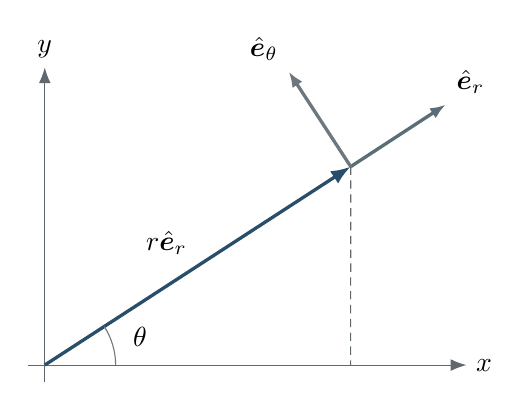
\begin{tikzpicture}[scale=1.05]
  \coordinate (O) at (0,0);
  \coordinate (P) at (3.7,2.4);
  \coordinate (X) at (3.7,0);
  \draw[axis] (-0.2,0)--(5.1,0) node[right] {$x$};
  \draw[axis] (0,-0.2)--(0,3.6) node[above] {$y$};
  \draw[vector] (O)--(P) node[midway,above left] {$r\uvec e_r$};
  \draw[axis,draw=Green,very thick] (P)--++(1.15,0.75) node[above right] {$\uvec e_r$};
  \draw[axis,draw=Gold,very thick] (P)--++(-0.75,1.15) node[above left] {$\uvec e_\theta$};
  \draw[guide] (P)--(3.7,0);
  \pic[draw=Gold,angle radius=9mm,angle eccentricity=1.4,"$\theta$"] {angle=X--O--P};
\end{tikzpicture}
\end{center}

与固定的 $\uvec e_x,\uvec e_y$ 不同，$\uvec e_r,\uvec e_\theta$ 会随方位改变。利用上一小节
已经建立的链式法则，对时间逐步求导：
\begin{align*}
  \frac{\dd\uvec e_r}{\dd t}
  &=\frac{\dd}{\dd t}(\cos\theta,\sin\theta)
    =(-\sin\theta\,\dot\theta,\cos\theta\,\dot\theta)
    =\dot\theta\,\uvec e_\theta,\\
  \frac{\dd\uvec e_\theta}{\dd t}
  &=\frac{\dd}{\dd t}(-\sin\theta,\cos\theta)
    =(-\cos\theta\,\dot\theta,-\sin\theta\,\dot\theta)
    =-\dot\theta\,\uvec e_r.
\end{align*}
因此
\begin{equation}
  \frac{\dd\uvec e_r}{\dd t}=\dot\theta\,\uvec e_\theta,
  \qquad
  \frac{\dd\uvec e_\theta}{\dd t}=-\dot\theta\,\uvec e_r.
  \label{eq:polar-basis-derivative}
\end{equation}

位置矢量为 $\vect r=r\uvec e_r$。用乘积法则求导：
\begin{align*}
  \vect v
  &=\frac{\dd}{\dd t}(r\uvec e_r)
    =\dot r\,\uvec e_r+r\frac{\dd\uvec e_r}{\dd t}\\
  &=\dot r\,\uvec e_r+r\dot\theta\,\uvec e_\theta.
\end{align*}
故
\begin{equation}
  \vect v=\dot r\,\uvec e_r+r\dot\theta\,\uvec e_\theta.
  \label{eq:polar-velocity}
\end{equation}
再对速度的两项分别使用乘积法则：
\begin{align*}
  \vect a
  &=\frac{\dd}{\dd t}(\dot r\,\uvec e_r)
    +\frac{\dd}{\dd t}(r\dot\theta\,\uvec e_\theta)\\
  &=\ddot r\,\uvec e_r+\dot r\dot\theta\,\uvec e_\theta
    +(\dot r\dot\theta+r\ddot\theta)\uvec e_\theta
    -r\dot\theta^2\uvec e_r\\
  &=(\ddot r-r\dot\theta^2)\uvec e_r
    +(r\ddot\theta+2\dot r\dot\theta)\uvec e_\theta.
\end{align*}
由此得到
\begin{equation}
  \vect a
  =\left(\ddot r-r\dot\theta^2\right)\uvec e_r
  +\left(r\ddot\theta+2\dot r\dot\theta\right)\uvec e_\theta.
  \label{eq:polar-acceleration}
\end{equation}
其中 $-r\dot\theta^2$ 是向心项，$r\ddot\theta$ 是切向角加速项；
$2\dot r\dot\theta$ 是由径向运动和转动共同产生的几何耦合项，有时称为科里奥利型项。
这里是在惯性系中分解加速度，不能把它直接解释成一种额外的惯性力。

\begin{examplebox}{匀速圆周运动为何仍有加速度}
半径为 $R$ 的质点以恒定角速度 $\omega$ 做圆周运动。用极坐标写出速度和加速度。

\tcblower
此时
\[
  r=R,\quad \dot r=\ddot r=0,\quad
  \dot\theta=\omega,\quad \ddot\theta=0.
\]
代入式 \eqref{eq:polar-velocity}、\eqref{eq:polar-acceleration}：
\[
  \vect v=R\omega\,\uvec e_\theta,
  \qquad
  \vect a=-R\omega^2\,\uvec e_r.
\]
速度大小不变，但基矢 $\uvec e_\theta$ 的方向持续改变，因此仍有指向圆心的加速度。
\end{examplebox}

\begin{examplebox}{沿阿基米德螺线运动}
质点的极坐标满足 $r=ct$、$\theta=\omega t$，其中 $c>0$、$\omega$ 为常量。求速度和
加速度，并解释各分量的来源。

\tcblower
由已知关系
\[
  \dot r=c,\qquad \ddot r=0,\qquad
  \dot\theta=\omega,\qquad \ddot\theta=0.
\]
代入极坐标公式：
\[
  \vect v=c\,\uvec e_r+c\omega t\,\uvec e_\theta,
  \qquad
  \vect a=-c\omega^2t\,\uvec e_r+2c\omega\,\uvec e_\theta.
\]
虽然 $\dot r$ 与 $\dot\theta$ 都是常量，加速度并不为零。径向项来自随半径增大的向心加速度，
横向项来自径向运动与转动的耦合；只对两个数值分量分别求导会漏掉基矢变化。
\end{examplebox}

\begin{warningbox}{极坐标基矢不能当作常量}
对 $r\uvec e_r$ 求导时若漏掉 $r\,\dd\uvec e_r/\dd t$，就会丢失横向速度；再次求导时若把
基矢当常量，就会同时丢失向心项和 $2\dot r\dot\theta$ 项。
\end{warningbox}

\begin{examplebox}{用极坐标建立单摆方程}
质量为 $m$ 的小球通过长为 $\ell$ 的轻绳悬挂，摆角 $\theta$ 从竖直向下方向量起。
忽略空气阻力，写出径向和切向运动方程。

\tcblower
取 $\uvec e_r$ 从悬点指向小球，$\uvec e_\theta$ 沿 $\theta$ 增大的方向。绳长不变给出
\[
  r=\ell,\qquad \dot r=0,\qquad \ddot r=0,
\]
所以
\begin{equation}
  \vect a=-\ell\dot\theta^2\uvec e_r
  +\ell\ddot\theta\uvec e_\theta.
  \label{eq:pendulum-polar-acceleration}
\end{equation}
张力为 $-T\uvec e_r$，重力的两个有符号分量为
\[
  m\vect g\cdot\uvec e_r=mg\cos\theta,
  \qquad
  m\vect g\cdot\uvec e_\theta=-mg\sin\theta.
\]
把牛顿第二定律分别投影，得到
\begin{align}
  mg\cos\theta-T&=-m\ell\dot\theta^2,
  \label{eq:pendulum-radial}\\
  -mg\sin\theta&=m\ell\ddot\theta.
  \label{eq:pendulum-tangential}
\end{align}
因此
\[
  T=mg\cos\theta+m\ell\dot\theta^2,
  \qquad
  \ddot\theta+\frac{g}{\ell}\sin\theta=0.
\]
当 $|\theta|\ll1$ 时，$\sin\theta\approx\theta$，后一方程线性化为
$\ddot\theta+(g/\ell)\theta=0$。径向方程决定张力，切向方程决定摆角演化，约束力因而
不会进入摆角的运动方程。
\end{examplebox}

\subsection{积分：从微元求和到连续积累}

设要累积区间 $[a,b]$ 上由函数 $f(x)$ 描述的贡献。把区间分成 $N$ 段，
$\Delta x=(b-a)/N$，在第 $i$ 段取一点 $\xi_i$。若每一小段内函数变化可以忽略，
该段贡献近似为 $f(\xi_i)\Delta x$，总贡献近似为
\[
  S_N=\sum_{i=1}^{N}f(\xi_i)\Delta x.
\]
令分割无限加细，就得到定积分
\begin{equation}
  \int_a^b f(x)\,\dd x
  =\lim_{N\to\infty}\sum_{i=1}^{N}f(\xi_i)\Delta x.
  \label{eq:riemann-integral}
\end{equation}
积分不是把“无穷小量”当普通数字相加，而是有限和在分割尺度趋近于零时的极限。

\begin{center}
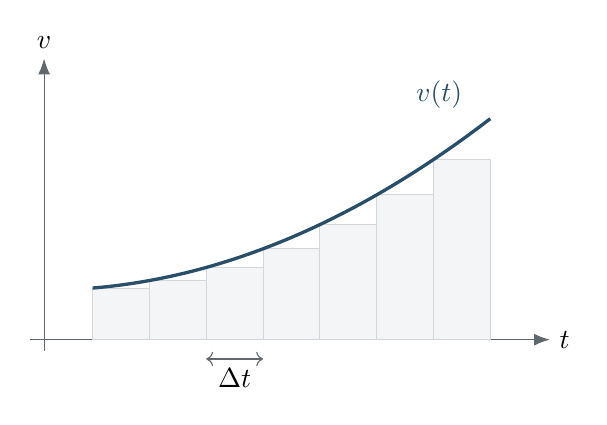
\begin{tikzpicture}[x=0.88cm,y=0.70cm]
  \draw[axis] (-0.2,0)--(7.3,0) node[right] {$t$};
  \draw[axis] (0,-0.2)--(0,5.1) node[above] {$v$};
  \foreach \i in {0,...,6}{
    \pgfmathsetmacro{\xleft}{0.7+0.82*\i}
    \pgfmathsetmacro{\height}{0.9+0.075*(\xleft)*(\xleft)}
    \draw[fill=PaleBlue,draw=RuleGray]
      (\xleft,0) rectangle ++(0.82,\height);
  }
  \draw[curve,domain=0.7:6.44,samples=80]
    plot (\x,{0.9+0.075*(\x)*(\x)});
  \node[DeepBlue] at (5.7,4.45) {$v(t)$};
  \draw[<->,draw=TextGray] (2.34,-0.35)--(3.16,-0.35)
    node[midway,below] {$\Delta t$};
\end{tikzpicture}
\end{center}

导数和积分的互逆关系可以直接从“累积量”看出。定义
\[
  F(x)=\int_a^x f(u)\,\dd u.
\]
当上限从 $x$ 增加到 $x+h$ 时，新增面积为 $\int_x^{x+h}f(u)\dd u$，所以
\[
  \frac{F(x+h)-F(x)}{h}
  =\frac1h\int_x^{x+h}f(u)\,\dd u.
\]
若 $f$ 连续，$h\to0$ 时右侧趋近 $f(x)$，于是
\begin{equation}
  \frac{\dd}{\dd x}\int_a^x f(u)\,\dd u=f(x),
  \qquad
  \int_a^b f(x)\,\dd x=F(b)-F(a).
  \label{eq:fundamental-theorem}
\end{equation}
这就是微积分基本定理。

\begin{warningbox}{定积分是有符号的累积量}
若 $f(x)<0$，相应小段对积分作负贡献。因此位移
$\int v\dd t$ 可以小于路程，变力做功也可能为负。只有在被积函数非负时，定积分才直接
等于通常所说的几何面积。
\end{warningbox}

\subsection{运动学中的积分关系}

由 $v=\dd x/\dd t$、$a=\dd v/\dd t$，可以写出微分形式
\[
  \dd x=v(t)\,\dd t,
  \qquad
  \dd v=a(t)\,\dd t.
\]
在给定时间区间上积分，得到
\begin{equation}
  x(t)-x(t_0)=\int_{t_0}^{t}v(\tau)\,\dd\tau,
  \qquad
  v(t)-v(t_0)=\int_{t_0}^{t}a(\tau)\,\dd\tau.
  \label{eq:kinematic-integrals}
\end{equation}
积分变量写成 $\tau$ 是为了避免与积分上限 $t$ 混淆；它只是积分过程中的哑变量。

\begin{examplebox}{随时间线性减小的加速度}
质点在 $0\le t\le T$ 内的加速度为
\[
  a(t)=a_0\left(1-\frac{t}{T}\right),
\]
且 $x(0)=0,v(0)=0$。求 $v(t),x(t)$ 以及 $t=T$ 时的速度和位移。

\tcblower
先积累加速度：
\begin{align*}
  v(t)
  &=\int_0^t a_0\left(1-\frac{\tau}{T}\right)\dd\tau\\
  &=a_0\left(t-\frac{t^2}{2T}\right).
\end{align*}
再积累速度：
\begin{align*}
  x(t)
  &=\int_0^t a_0\left(\tau-\frac{\tau^2}{2T}\right)\dd\tau\\
  &=a_0\left(\frac{t^2}{2}-\frac{t^3}{6T}\right).
\end{align*}
所以
\[
  v(T)=\frac12a_0T,
  \qquad
  x(T)=\frac13a_0T^2.
\]
量纲分别为速度和长度；同时 $a(t)\ge0$，所以 $v(t)$ 在区间内应单调增加，结果与此一致。
\end{examplebox}

若加速度以位置的函数 $a(x)$ 给出，直接对时间积分并不方便。用链式法则
\begin{equation}
  a=\frac{\dd v}{\dd t}
  =\frac{\dd v}{\dd x}\frac{\dd x}{\dd t}
  =v\frac{\dd v}{\dd x},
  \label{eq:a-vdvdx}
\end{equation}
于是
\begin{equation}
  v\,\dd v=a(x)\,\dd x,
  \qquad
  \frac12(v^2-v_0^2)=\int_{x_0}^{x}a(\xi)\,\dd\xi.
  \label{eq:position-dependent-acceleration}
\end{equation}
当 $a$ 为常量时，立即得到 $v^2=v_0^2+2a(x-x_0)$。这说明熟悉的运动学公式
只是一般积分关系的一个特例。

把变化率关系与初始条件结合，便会进入微分方程的求解。线性阻力、平方阻力和指数衰变
将在下一节集中比较，这里不提前重复求解。

\subsection{变力做功与动能定理}

一维运动中，物体发生微小位移 $\dd x$ 时，力 $F(x)$ 所做的元功为
\[
  \dd W=F(x)\,\dd x.
\]
从 $x_1$ 到 $x_2$，该力所做的功为
\begin{equation}
  W_{1\to2}=\int_{x_1}^{x_2}F(x)\,\dd x.
  \label{eq:variable-force-work}
\end{equation}
若力与位移方向相反，$F$ 在所选正方向上的分量为负，积分自然给出负功。

动能定理讨论的是所有力所做的总功。令 $F_{\mathrm{net}}(x)$ 表示物体所受合力，
利用牛顿第二定律 $F_{\mathrm{net}}=ma$ 和式 \eqref{eq:a-vdvdx}：
\begin{align*}
  W_{\mathrm{net},1\to2}
  &=\int_{x_1}^{x_2}F_{\mathrm{net}}(x)\,\dd x
  =\int_{x_1}^{x_2}ma\,\dd x
  =\int_{x_1}^{x_2}m v\frac{\dd v}{\dd x}\,\dd x\\
  &=\int_{v_1}^{v_2}mv\,\dd v
  =\frac12mv_2^2-\frac12mv_1^2.
\end{align*}
因此
\begin{equation}
  W_{\mathrm{net},1\to2}=\Delta K.
  \label{eq:work-energy-theorem}
\end{equation}
三维情形中，动能定理对应的元功应写成
$\dd W_{\mathrm{net}}=\vect F_{\mathrm{net}}\cdot\dd\vect r$。

\begin{examplebox}{弹簧力做功与势能}
弹簧沿 $x$ 轴放置，平衡位置为 $x=0$，弹簧力为 $F=-kx$。求物体从 $x_1$
移动到 $x_2$ 时弹簧力所做的功，并由此写出弹性势能。

\tcblower
由变力做功定义
\begin{align*}
  W_{1\to2}
  &=\int_{x_1}^{x_2}(-kx)\,\dd x
  =-\frac12k(x_2^2-x_1^2)\\
  &=\frac12kx_1^2-\frac12kx_2^2.
\end{align*}
保守力做功等于势能减少量 $W_{1\to2}=U(x_1)-U(x_2)$，所以可取
\begin{equation}
  U(x)=\frac12kx^2+C.
  \label{eq:spring-potential}
\end{equation}
势能零点可以任意选择，常取 $C=0$。对势能求导又得到
\[
  -\frac{\dd U}{\dd x}=-kx=F,
\]
这说明“由力积分得到势能”与“由势能求导得到力”互为逆过程。
\end{examplebox}

\subsection{连续分布与微元建模}

当质量、电荷或其他物理量连续分布时，先选取适合对称性和几何形状的微元。例如细杆的
线密度为 $\lambda(x)$，长度元 $\dd x$ 上的质量为
\[
  \dd m=\lambda(x)\,\dd x.
\]
因此总质量和质心位置分别为
\begin{equation}
  M=\int\dd m,
  \qquad
  x_{\mathrm{cm}}=\frac1M\int x\,\dd m.
  \label{eq:continuous-center-of-mass}
\end{equation}
面分布使用 $\dd m=\sigma\,\dd S$，体分布使用 $\dd m=\rho\,\dd V$。密度和微元必须
匹配：线密度不能直接乘面积元，体密度也不能直接乘长度元。

\begin{examplebox}{非均匀细杆的质心}
一根细杆占据 $0\le x\le L$，线密度为
\[
  \lambda(x)=\lambda_0\left(1+\frac{x}{L}\right).
\]
求总质量和质心位置。

\tcblower
质量微元为 $\dd m=\lambda(x)\dd x$，故
\begin{align*}
  M
  &=\int_0^L\lambda_0\left(1+\frac{x}{L}\right)\dd x
  =\lambda_0\left(L+\frac L2\right)
  =\frac32\lambda_0L.
\end{align*}
关于原点的一阶矩为
\begin{align*}
  \int_0^Lx\,\dd m
  &=\lambda_0\int_0^L\left(x+\frac{x^2}{L}\right)\dd x\\
  &=\lambda_0\left(\frac{L^2}{2}+\frac{L^2}{3}\right)
  =\frac56\lambda_0L^2.
\end{align*}
所以
\[
  x_{\mathrm{cm}}
  =\frac{(5/6)\lambda_0L^2}{(3/2)\lambda_0L}
  =\frac59L.
\]
由于线密度随 $x$ 增大，质心应位于中点 $L/2$ 的右侧；$5L/9$ 符合这一物理判断。
\end{examplebox}

以上讨论的微元都沿固定坐标轴选取。曲线弧长和沿路径运动时间还需要建立几何微元
$\dd s$，将在第五节从折线极限开始专门推导，这里只保留连续分布的基本建模方法。

\subsection*{分层训练}
\begin{enumerate}[label=\textbf{\arabic*.},leftmargin=2.4em]
  \item \textbf{基础} 已知 $x(t)=A(1-\e^{-t/\tau})$。求速度和加速度，并由
  $t\ll\tau$ 的展开说明运动初期的速度近似为何值。
  \item \textbf{方法} 质点满足 $r=r_0\e^{kt}$、$\theta=\omega t$。求极坐标形式的
  $\vect v$ 与 $\vect a$，并分别解释两个加速度分量。
  \item \textbf{方法} 质量为 $m$ 的质点在稳定平衡点附近的势能可写成
  $U(x)=U_0+\frac12\kappa x^2+\order{x^3}$。证明最低阶运动是简谐运动，并求角频率。
  \item \textbf{提升} 细杆占据 $0\le x\le L$，线密度
  $\lambda(x)=\lambda_0[1-(x/L)^2]$。求总质量和质心位置，并用密度分布判断结果方向是否合理。
\end{enumerate}
{\small\color{TextGray}\noindent
参考结果：$v=(A/\tau)\e^{-t/\tau}$，$a=-(A/\tau^2)\e^{-t/\tau}$，初期
$v\approx A/\tau$；$\vect v=kr\uvec e_r+\omega r\uvec e_\theta$，
$\vect a=(k^2-\omega^2)r\uvec e_r+2k\omega r\uvec e_\theta$；
$\omega_0=\sqrt{\kappa/m}$；$M=2\lambda_0L/3$，$x_{\rm cm}=3L/8$。\par}

\ifdefined\MASTERBOOK
  \let\sectionfinish\relax
\else
  \def\sectionfinish{\end{document}}
\fi
\sectionfinish
